\documentclass[border=5pt]{standalone}
\usepackage{tikz}
\begin{document}
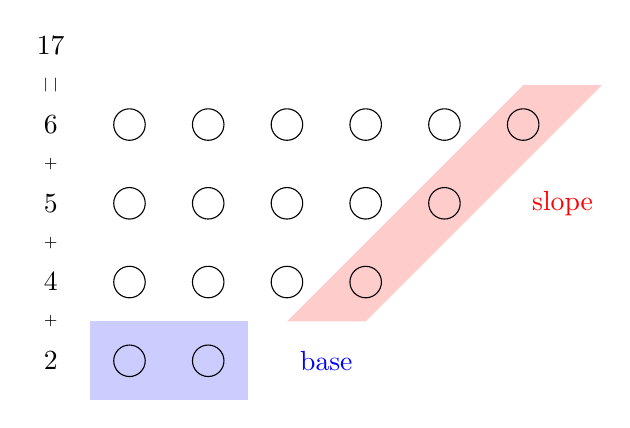
\begin{tikzpicture}[scale=1]
\fill[blue!20!white] (-0.5,-3.5)--(1.5,-3.5)--(1.5,-2.5)--(-0.5,-2.5);
\fill[red!20!white] (2.,-2.5)--(3.,-2.5)--(6.,0.5)--(5.,0.5);
\draw (5.5,-1) node{\color{red}slope};
\draw (2.5,-3) node{\color{blue}base};
\draw (-1,1) node{$17$};
\draw (-1,0.5) node{$\scriptscriptstyle\mid\,\mid$};
\draw (-1,0) node{$6$};
\draw (-1,-0.5) node{$\scriptscriptstyle+$};
\draw (0,0) circle(0.2 cm);
\draw (1,0) circle(0.2 cm);
\draw (2,0) circle(0.2 cm);
\draw (3,0) circle(0.2 cm);
\draw (4,0) circle(0.2 cm);
\draw (5,0) circle(0.2 cm);
\draw (-1,-1) node{$5$};
\draw (-1,-1.5) node{$\scriptscriptstyle+$};
\draw (0,-1) circle(0.2 cm);
\draw (1,-1) circle(0.2 cm);
\draw (2,-1) circle(0.2 cm);
\draw (3,-1) circle(0.2 cm);
\draw (4,-1) circle(0.2 cm);
\draw (-1,-2) node{$4$};
\draw (-1,-2.5) node{$\scriptscriptstyle+$};
\draw (0,-2) circle(0.2 cm);
\draw (1,-2) circle(0.2 cm);
\draw (2,-2) circle(0.2 cm);
\draw (3,-2) circle(0.2 cm);
\draw (-1,-3) node{$2$};
\draw (0,-3) circle(0.2 cm);
\draw (1,-3) circle(0.2 cm);
\end{tikzpicture}
\end{document}
